\documentclass[a4paper]{article}
\usepackage{amsmath,amsfonts,amsthm,amssymb}
\usepackage{tikz}
\usepackage{graphicx}
\usepackage{geometry}
\newcommand{\vv}{\mathbf}
\newcommand{\nul}{\mathrm{null}}
\newcommand{\spa}{\mathrm{span}}
\newcommand{\adj}{\mathrm{adj}}
\title{Application of Diagonalisation: Markov Chain}
\author{Gordon Chan}


%\usetikzlibrary{shapes,arrows,positioning}
\usetikzlibrary{automata,arrows,positioning,calc}


\begin{document}
\maketitle
Suppose there are two states, 1 and 2. The probabilities of change of state can be summarised by the diagram below:
\begin{center}
	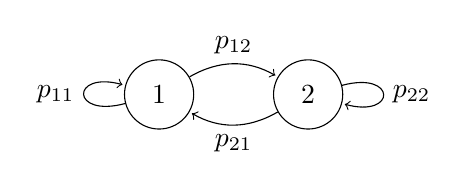
\begin{tikzpicture}
		% Draw the states
        	\node[state]             (1) {1};
        	\node[state, right=of 1] (2) {2};

        	% Connect the states with arrows
        	\draw[every loop]
			(1) edge[bend left, auto=left] node {\(p_{12}\)} (2)
			(2) edge[bend left, auto=left] node {\(p_{21}\)} (1)
			(1) edge[loop left] node {\(p_{11}\)} (1)
			(2) edge[loop right] node {\(p_{22}\)} (2);
	\end{tikzpicture}
\end{center}

This can be represented by the matrix \(\vv P\).
\[\vv P=\begin{bmatrix}
	p_{11}&p_{12}\\
	p_{21}&p_{22}
\end{bmatrix}\]

Let \(p_{12}\) and \(p_{21}\) be \(a\) and \(b\) respectively, where \(a,b\in(0,1)\). For ease of calculations, let \(\vv A\) be the transpose of \(\vv P\), such that:

\[\vv A=\vv P^{\mathrm T}=
\begin{bmatrix}
	p_{11}&p_{21}\\
	p_{12}&p_{22}
\end{bmatrix}=
\begin{bmatrix}
	1-a&b\\
	a&1-b
\end{bmatrix}\]

Let \(\lambda\) be the eigenvalues of \(\vv A\). \(\forall\vv v\in\mathbb R^2\backslash\{\vv0\}\),
\[\begin{aligned}
	\lambda\vv v&=\vv A\vv v\\
	\lambda\vv v-\vv A\vv v&=\vv0\\
	(\lambda\vv I-\vv A)\vv v&=\vv0\\
	\det(\lambda\vv I-\vv A)&=0\\
	\begin{vmatrix}
		\lambda+a-1&-b\\
		-a&\lambda+b-1
	\end{vmatrix}&=0\\
	(\lambda+a-1)(\lambda+b-1)-(-b)(-a)&=0\\
	\lambda^2+b\lambda-\lambda+a\lambda+ab-a-\lambda-b+1-ab&=0\\
	\lambda^2+(a+b-2)\lambda+1-a-b&=0\\
\end{aligned}\]

Let the discriminant of the quadratic in \(\lambda\) be \(\Delta\).
\[\begin{aligned}
	\Delta&=(a+b-2)^2-4(1)(1-a-b)\\
	      &=a^2+ab-2a+ab+b^2-2b-2a-2b+4-4+4a+4b\\
	      &=a^2+2ab+b^2\\
	      &=(a+b)^2
\end{aligned}\]

\[\lambda=\frac{-(a+b-2)\pm\sqrt{\Delta}}{2(1)}=\frac{2-a-b\pm(a+b)}{2}\]
\[\lambda\in\{1,1-a-b\}\]

For \(\lambda=1\),
\[\begin{aligned}
	(\lambda\vv I-\vv A)\vv x&=\vv0\\
	\begin{bmatrix}
		a&-b\\
		-a&b
	\end{bmatrix}\vv x
				 &=\vv0\\
	\begin{bmatrix}
		a&-b\\
		0&0
	\end{bmatrix}\vv x
				 &=\vv0\\
	\begin{bmatrix}
		a&-b\\
		0&0
	\end{bmatrix}\vv x
				 &=\vv0\\
	ax_1-bx_2&=0\\
	ax_1&=bx_2\\
	x_1&=\frac bax_2
\end{aligned}\]

Let \(x_2=k\). \(x_1=\frac bak\).
\[\vv x=\begin{bmatrix}\frac bak\\k\end{bmatrix}=bk\begin{bmatrix}b\\a\end{bmatrix}\]
\[\nul(\vv I-\vv A)=\spa\left\{\begin{bmatrix}b\\a\end{bmatrix}\right\}\]

For \(\lambda=1-a-b\),
\[\begin{aligned}
	(\lambda\vv I-\vv A)\vv x&=\vv0\\
	\begin{bmatrix}
		-b&-b\\
		-a&-a
	\end{bmatrix}\vv x
				 &=\vv0\\
	\begin{bmatrix}
		1&1\\
		1&1
	\end{bmatrix}\vv x
				 &=\vv0\\
	\begin{bmatrix}
		1&1\\
		0&0
	\end{bmatrix}\vv x
				 &=\vv0\\
	x_1+x_2&=0\\
	x_1&=-x_2
\end{aligned}\]

Let \(x_2=k\). \(x_1=-k\).
\[\vv x=\begin{bmatrix}-k\\k\end{bmatrix}=-k\begin{bmatrix}1\\-1\end{bmatrix}\]
\[\nul((1-a-b)\vv I-\vv A)=\spa\left\{\begin{bmatrix}1\\-1\end{bmatrix}\right\}\]

Let \(\vv A=\vv Q\vv D\vv Q^{-1}\).
\[\vv D=\begin{bmatrix}1&0\\0&1-a-b\end{bmatrix}\]
\[\vv Q=\begin{bmatrix}b&1\\a&-1\end{bmatrix}\]

Check:
\[\begin{aligned}
	\vv A\vv Q&=\vv A
	\begin{bmatrix}
		b&1\\
		a&-1
	\end{bmatrix}\\
		  &=
	\begin{bmatrix}
		\vv A\begin{bmatrix}b\\a\end{bmatrix}&\vv A\begin{bmatrix}1\\-1\end{bmatrix}\end{bmatrix}\\
						     &=
						     \begin{bmatrix}
		1\begin{bmatrix}b\\a\end{bmatrix}&(1-a-b)\begin{bmatrix}1\\-1\end{bmatrix}
	\end{bmatrix}\\
						     &=
	\begin{bmatrix}
		b&1\\
		a&-1
	\end{bmatrix}
	\begin{bmatrix}
		1&0\\
		0&1-a-b
	\end{bmatrix}\\
						     &=\vv Q\vv D
\end{aligned}\]

\[\vv A\vv Q=\vv Q\vv D\iff\vv A=\vv Q\vv D\vv Q^{-1}\]

\[\vv Q^{-1}=\frac{\adj(\vv Q)}{\det(\vv Q)}=\frac1{-b-a}\begin{bmatrix}-1&-1\\-a&b\end{bmatrix}=\frac1{a+b}\begin{bmatrix}1&1\\a&-b\end{bmatrix}\]

To find to equilibrium distribution of states, \(\lim\limits_{n\to\infty}\vv A^n\) is wanted.
\[\lim\limits_{n\to\infty}\vv D^n
	=\lim\limits_{n\to\infty}\begin{bmatrix}1&0\\0&1-a-b\end{bmatrix}^n
	=\lim\limits_{n\to\infty}\begin{bmatrix}1^n&0\\0&(1-a-b)^n\end{bmatrix}
	=\begin{bmatrix}1&0\\0&0\end{bmatrix}\]

\[\begin{aligned}
	\lim\limits_{n\to\infty}\vv A^n
	&=\lim\limits_{n\to\infty}\left(\vv Q\vv D\vv Q^{-1}\right)^n\\
	&=\lim\limits_{n\to\infty}\vv Q\vv D^n\vv Q^{-1}\\
	&=\vv Q\left(\lim\limits_{n\to\infty}\vv D^n\right)\vv Q^{-1}\\
	&=
	\begin{bmatrix}b&1\\a&-1\end{bmatrix}
	\begin{bmatrix}1&0\\0&0\end{bmatrix}
	\frac1{a+b}\begin{bmatrix}1&1\\a&-b\end{bmatrix}\\
	&=\frac1{a+b}
	\begin{bmatrix}b&1\\a&-1\end{bmatrix}
	\begin{bmatrix}1&0\\0&0\end{bmatrix}
	\begin{bmatrix}1&1\\a&-b\end{bmatrix}\\
	&=\frac1{a+b}
	\begin{bmatrix}b&1\\a&-1\end{bmatrix}
	\begin{bmatrix}1&1\\0&0\end{bmatrix}\\
	&=\frac1{a+b}
	\begin{bmatrix}b&b\\a&a\end{bmatrix}\\
			&=\begin{bmatrix}\frac b{a+b}&\frac b{a+b}\\\frac a{a+b}&\frac a{a+b}\end{bmatrix}\\
\end{aligned}\]

Let \(\vv s_0\) be the initial distribution of states.
It is obvious that.
\[\begin{aligned}
	s_1+s_2&=1\\
	s_1&=1-s_2
\end{aligned}\]
Let \(s_2=m\), \(s_1=1-m\).

The equilibrium distribution can be calculated as such:
\[\lim\limits_{n\to\infty}\vv s_n=\lim\limits_{n\to\infty}\vv A^n\vv s_0
=\left(\lim\limits_{n\to\infty}\vv A^n\right)\vv s_0
=\begin{bmatrix}\frac b{a+b}&\frac b{a+b}\\\frac a{a+b}&\frac a{a+b}\end{bmatrix}
\begin{bmatrix}1-m\\m\end{bmatrix}
=\begin{bmatrix}\frac b{a+b}\\\frac a{a+b}\end{bmatrix}
=\boxed{\begin{bmatrix}\frac {p_{21}}{p_{12}+p_{21}}\\\frac {p_{12}}{p_{12}+p_{21}}\end{bmatrix}}\]
\end{document}
